% This example is meant to be compiled with lualatex or xelatex
% The theme itself also supports pdflatex
\PassOptionsToPackage{unicode}{hyperref}
\documentclass[aspectratio=1610, 12pt]{beamer}

% Warning, if another latex run is needed
% \usepackage[aux]{rerunfilecheck}

% just list chapters and sections in the toc, not subsections or smaller
\setcounter{tocdepth}{1}

%------------------------------------------------------------------------------
%------------------------------ Fonts, Unicode, Language ----------------------
%------------------------------------------------------------------------------
\usepackage{fontspec}
\defaultfontfeatures{Ligatures=TeX}  % -- becomes en-dash etc.

% german language
\usepackage{polyglossia}
\setdefaultlanguage{german}

% for english abstract and english titles in the toc
\setotherlanguages{english}

% intelligent quotation marks, language and nesting sensitive
\usepackage[autostyle]{csquotes}

% microtypographical features, makes the text look nicer on the small scale
\usepackage{microtype}

%------------------------------------------------------------------------------
%------------------------ Math Packages and settings --------------------------
%------------------------------------------------------------------------------

\usepackage{amsmath}
\usepackage{amssymb}
\usepackage{mathtools}
\usepackage{bbold}

% Enable Unicode-Math and follow the ISO-Standards for typesetting math
\usepackage[
  math-style=ISO,
  bold-style=ISO,
  sans-style=italic,
  nabla=upright,
  partial=upright,
]{unicode-math}
\setmathfont{Latin Modern Math}

% nice, small fracs for the text with \sfrac{}{}
\usepackage{xfrac}


%------------------------------------------------------------------------------
%---------------------------- Numbers and Units -------------------------------
%------------------------------------------------------------------------------

\usepackage[
  locale=DE,
  separate-uncertainty=true,
  per-mode=symbol-or-fraction,
]{siunitx}
\sisetup{math-micro=\text{µ},text-micro=µ}
% \sisetup{tophrase={{ to }}}
%------------------------------------------------------------------------------
%-------------------------------- tables  -------------------------------------
%------------------------------------------------------------------------------

\usepackage{booktabs}       % \toprule, \midrule, \bottomrule, etc

%------------------------------------------------------------------------------
%-------------------------------- graphics -------------------------------------
%------------------------------------------------------------------------------

\usepackage{graphicx}
%\usepackage{rotating}
\usepackage{grffile}
\usepackage{tikz}
\usepackage{circuitikz}
\usepackage{tikz-feynman}
\usepackage{subcaption}

% allow figures to be placed in the running text by default:
\usepackage{scrhack}
\usepackage{float}
\floatplacement{figure}{htbp}
\floatplacement{table}{htbp}

% keep figures and tables in the section
\usepackage[section, below]{placeins}

% smileys
\usepackage{MnSymbol,wasysym}

%------------------------------------------------------------------------------
%---------------------- customize list environments ---------------------------
%------------------------------------------------------------------------------

\usepackage{enumitem}
\usepackage{listings}
\usepackage{hepunits}

\usepackage{pdfpages}
%------------------------------------------------------------------------------
%------------------------------ Bibliographie ---------------------------------
%------------------------------------------------------------------------------

\usepackage[
  backend=biber,   % use modern biber backend
  autolang=hyphen, % load hyphenation rules for if language of bibentry is not
                   % german, has to be loaded with \setotherlanguages
                   % in the references.bib use langid={en} for english sources
]{biblatex}
\addbibresource{references.bib}  % the bib file to use
\DefineBibliographyStrings{german}{andothers = {{et\,al\adddot}}}  % replace u.a. with et al.


% Load packages you need here
% \usepackage{polyglossia}
% \setmainlanguage{german}

\usepackage{csquotes}


% \usepackage{amsmath}
% \usepackage{amssymb}
% \usepackage{mathtools}

\usepackage{hyperref}
\usepackage{bookmark}

% load the theme after all packages

\usetheme[
  showtotalframes, % show total number of frames in the footline
]{tudo}

% Put settings here, like
\unimathsetup{
  math-style=ISO,
  bold-style=ISO,
  nabla=upright,
  partial=upright,
  mathrm=sym,
}

% \setbeamertemplate{itemize item}{\scriptsize$\blacktriangleright$}
% \setbeamertemplate{itemize subitem}{\scriptsize$\blacktriangleright$}

%Titel:
\title{Update: joint constraint tuning}
%\subtitle{tuning of uncertainties}
%Autor
\author[N.Breer]{Nils Breer}
%Lehrstuhl/Fakultät
\institute{TU Dortmund, AG Albrecht}
%\titlegraphic{\includegraphics[width=0.3\textwidth]{content/Bilder/interferenz.jpg}}
% \date{12.05.2023}

\begin{document}
\maketitle
% \setlength\itemsep{1em}
\begin{frame}
  \begin{columns}
    \begin{column}[c]{0.48\textwidth}
      \begin{itemize}
        \item loosen the Tx uncertainty (old ($1 \mu m$), $2 \mu m$, $10 \mu m$)
        \item 500k events, loose particle selection
        \item current uncertainties: 0.01 0.0012 0.0019 0.0004 0.00000047 0.00017 [mm, rad]
        \begin{itemize}
          \item tuned:  $\mu m, \chi^2$/dof: 1.02
          \item old: 1 $\mu m, \chi^2$/dof: 914.09
          \item 10 $\mu m, \chi^2$/dof: 55.49
          \item 2 $\mu m, \chi^2$/dof: 492.67
        \end{itemize}
      \end{itemize}
    \end{column}
    \begin{column}[c]{0.48\textwidth}
      $\chi^2$ probability vs. momentum
      \begin{figure}
        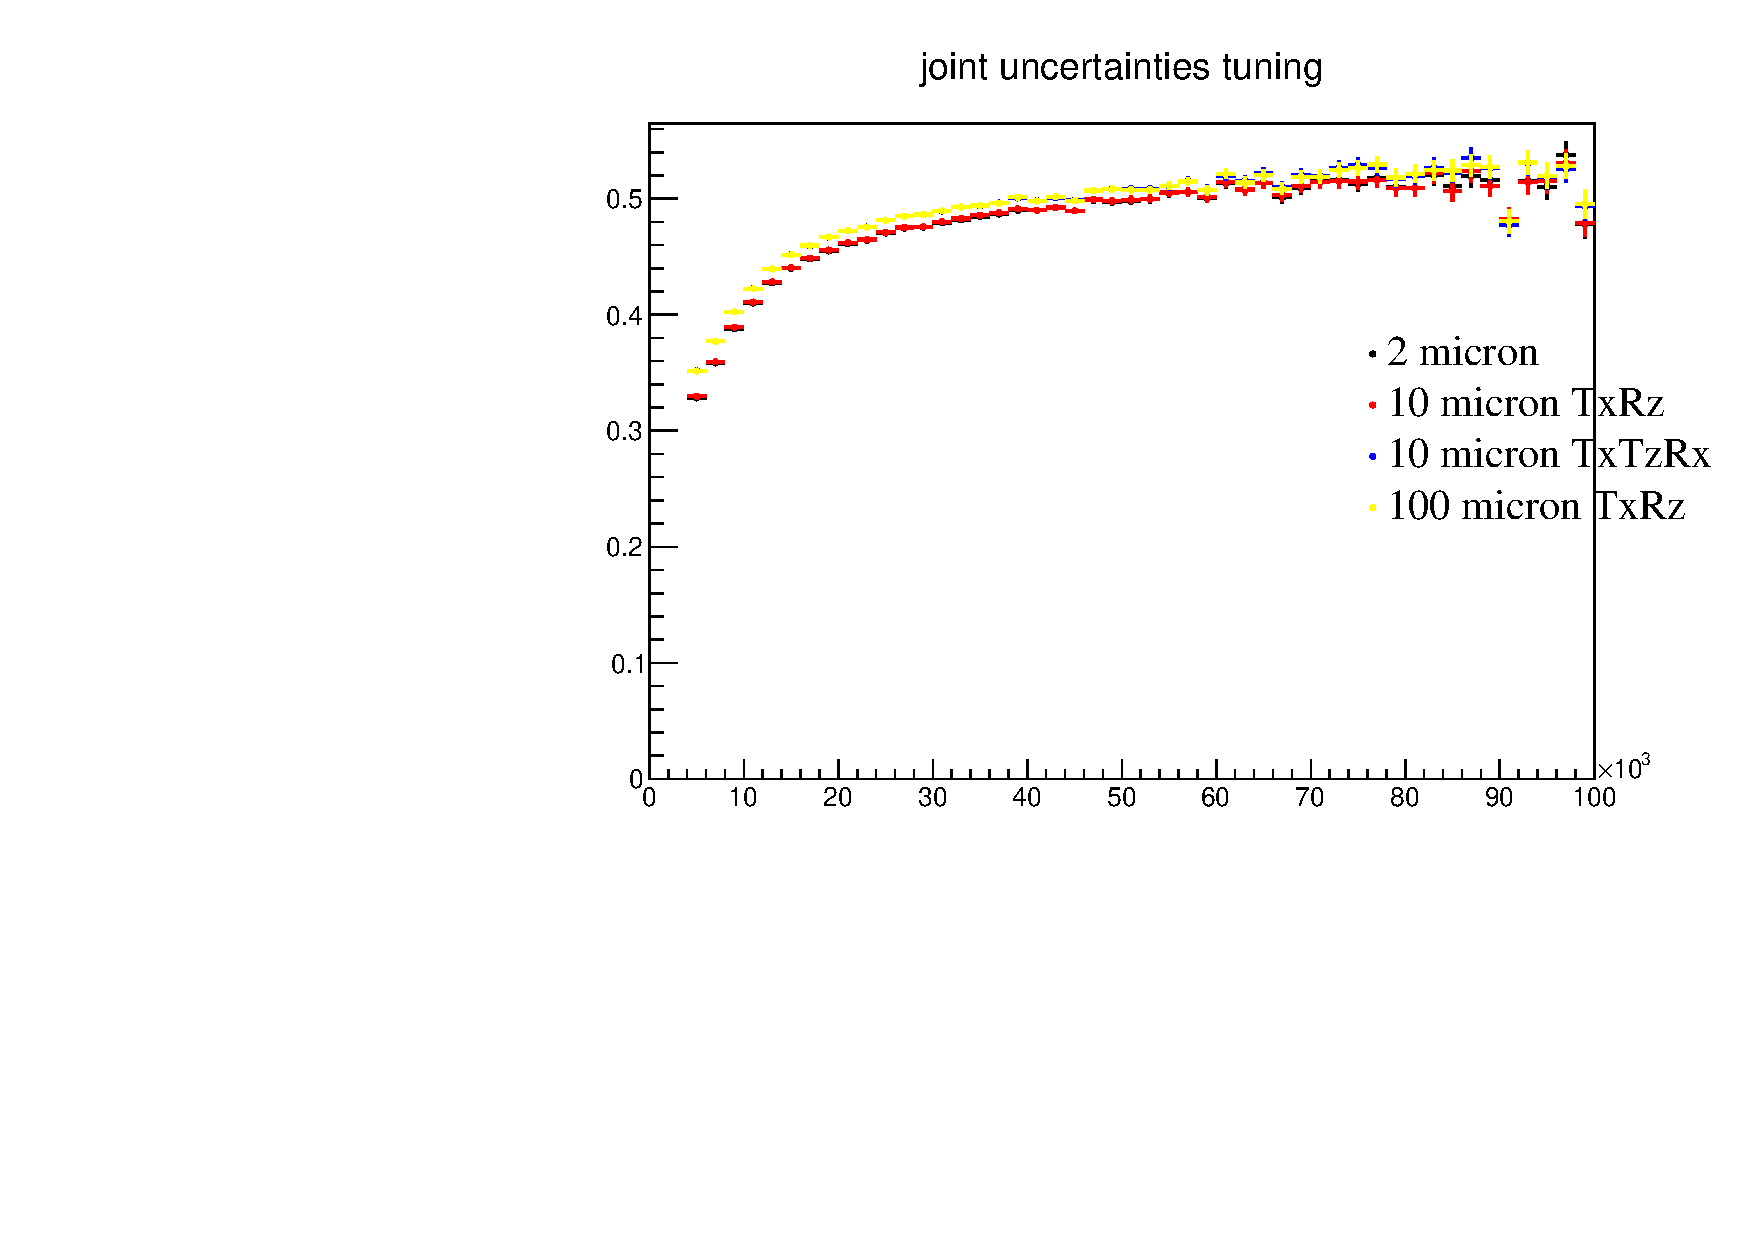
\includegraphics[width=\textwidth]{plots/compi/chi2ProbVsMom_comp_looser.pdf}
      \end{figure}
    \end{column}
  \end{columns}
\end{frame}

\begin{frame}
  \begin{columns}
    \begin{column}[c]{0.48\textwidth}
      $\chi^2$/dof
      \begin{figure}
        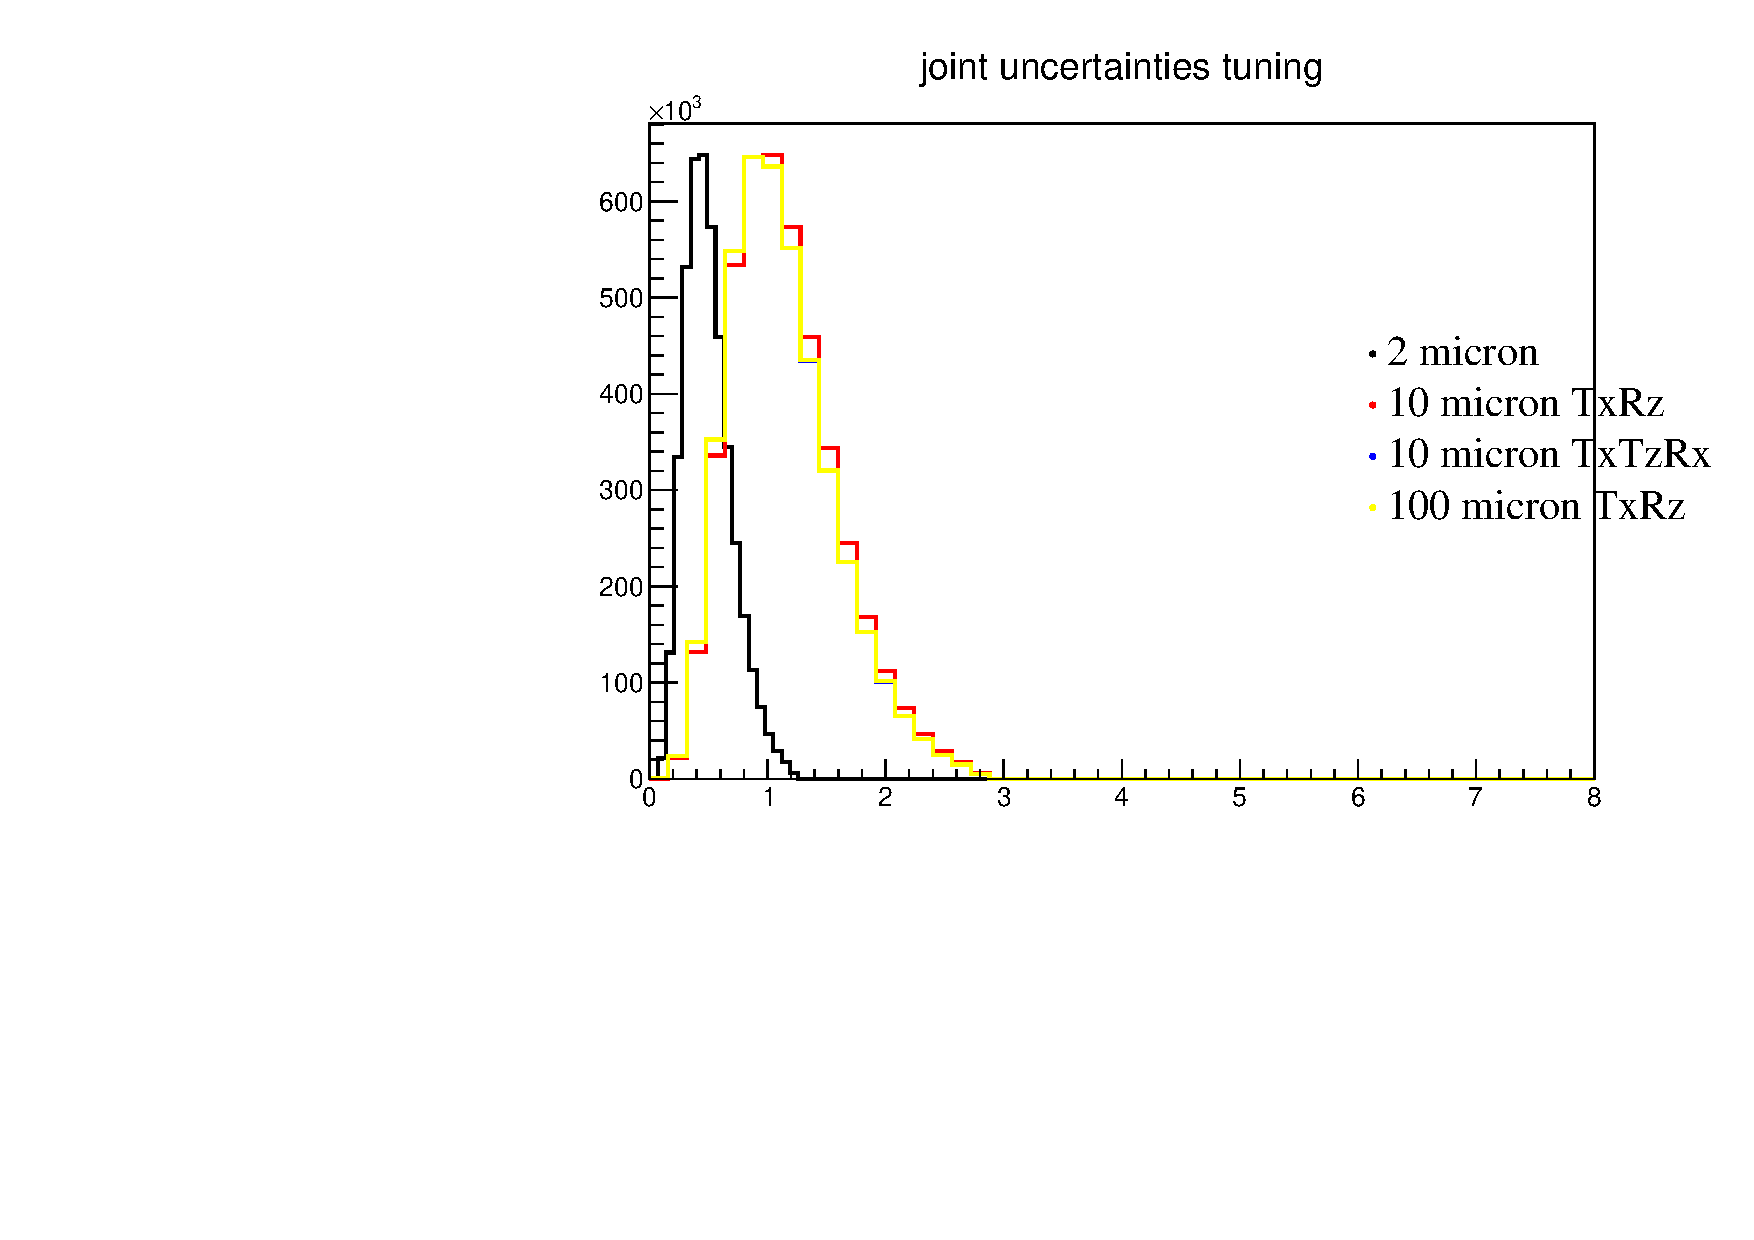
\includegraphics[width=\textwidth]{plots/compi/chi2_per_ndof_comp_looser.pdf}
      \end{figure}
    \end{column}
    \begin{column}[c]{0.48\textwidth}
      FTResidual
      \begin{figure}
        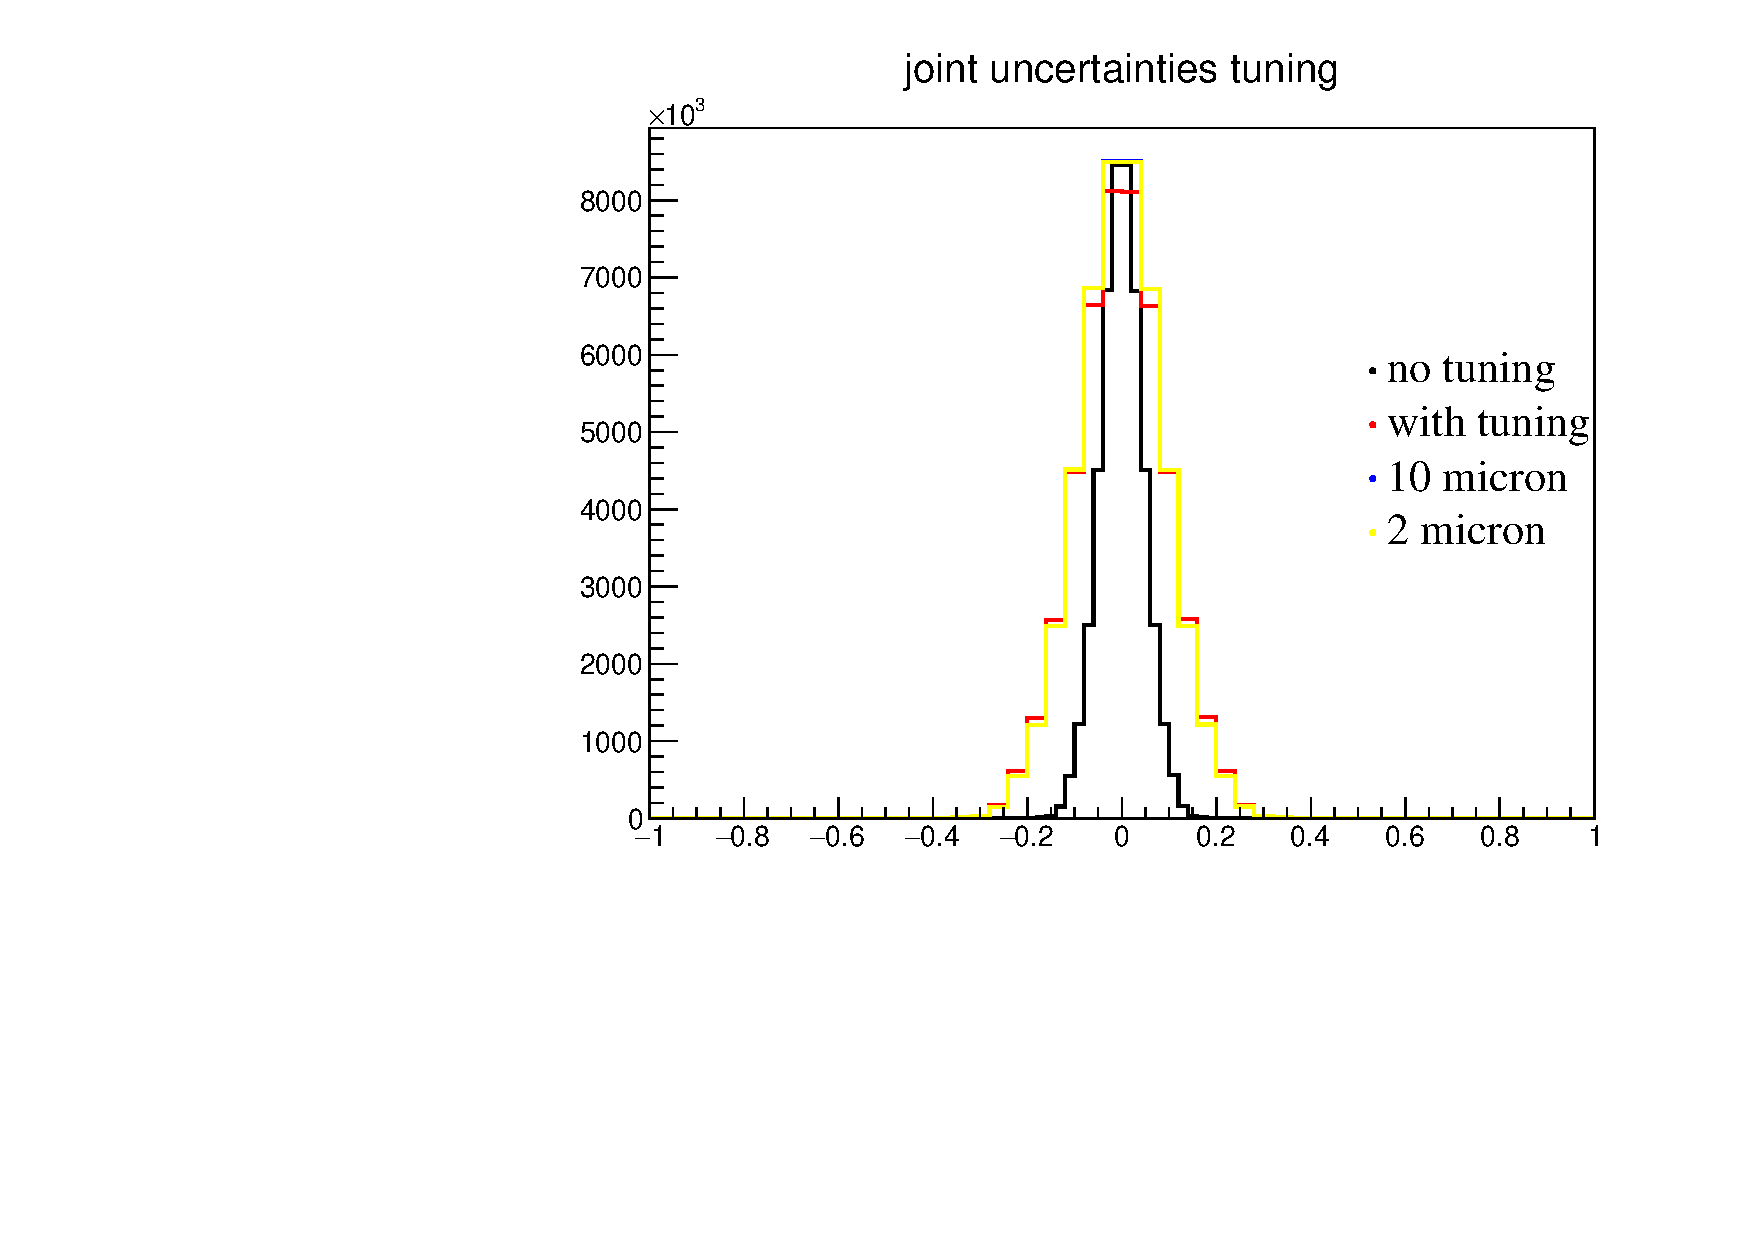
\includegraphics[width=\textwidth]{plots/compi/FTResidual_comp_looser.pdf}
      \end{figure}
    \end{column}
  \end{columns}
\end{frame}

\begin{frame}
  \begin{columns}
    \begin{column}[c]{0.48\textwidth}
      \begin{figure}
        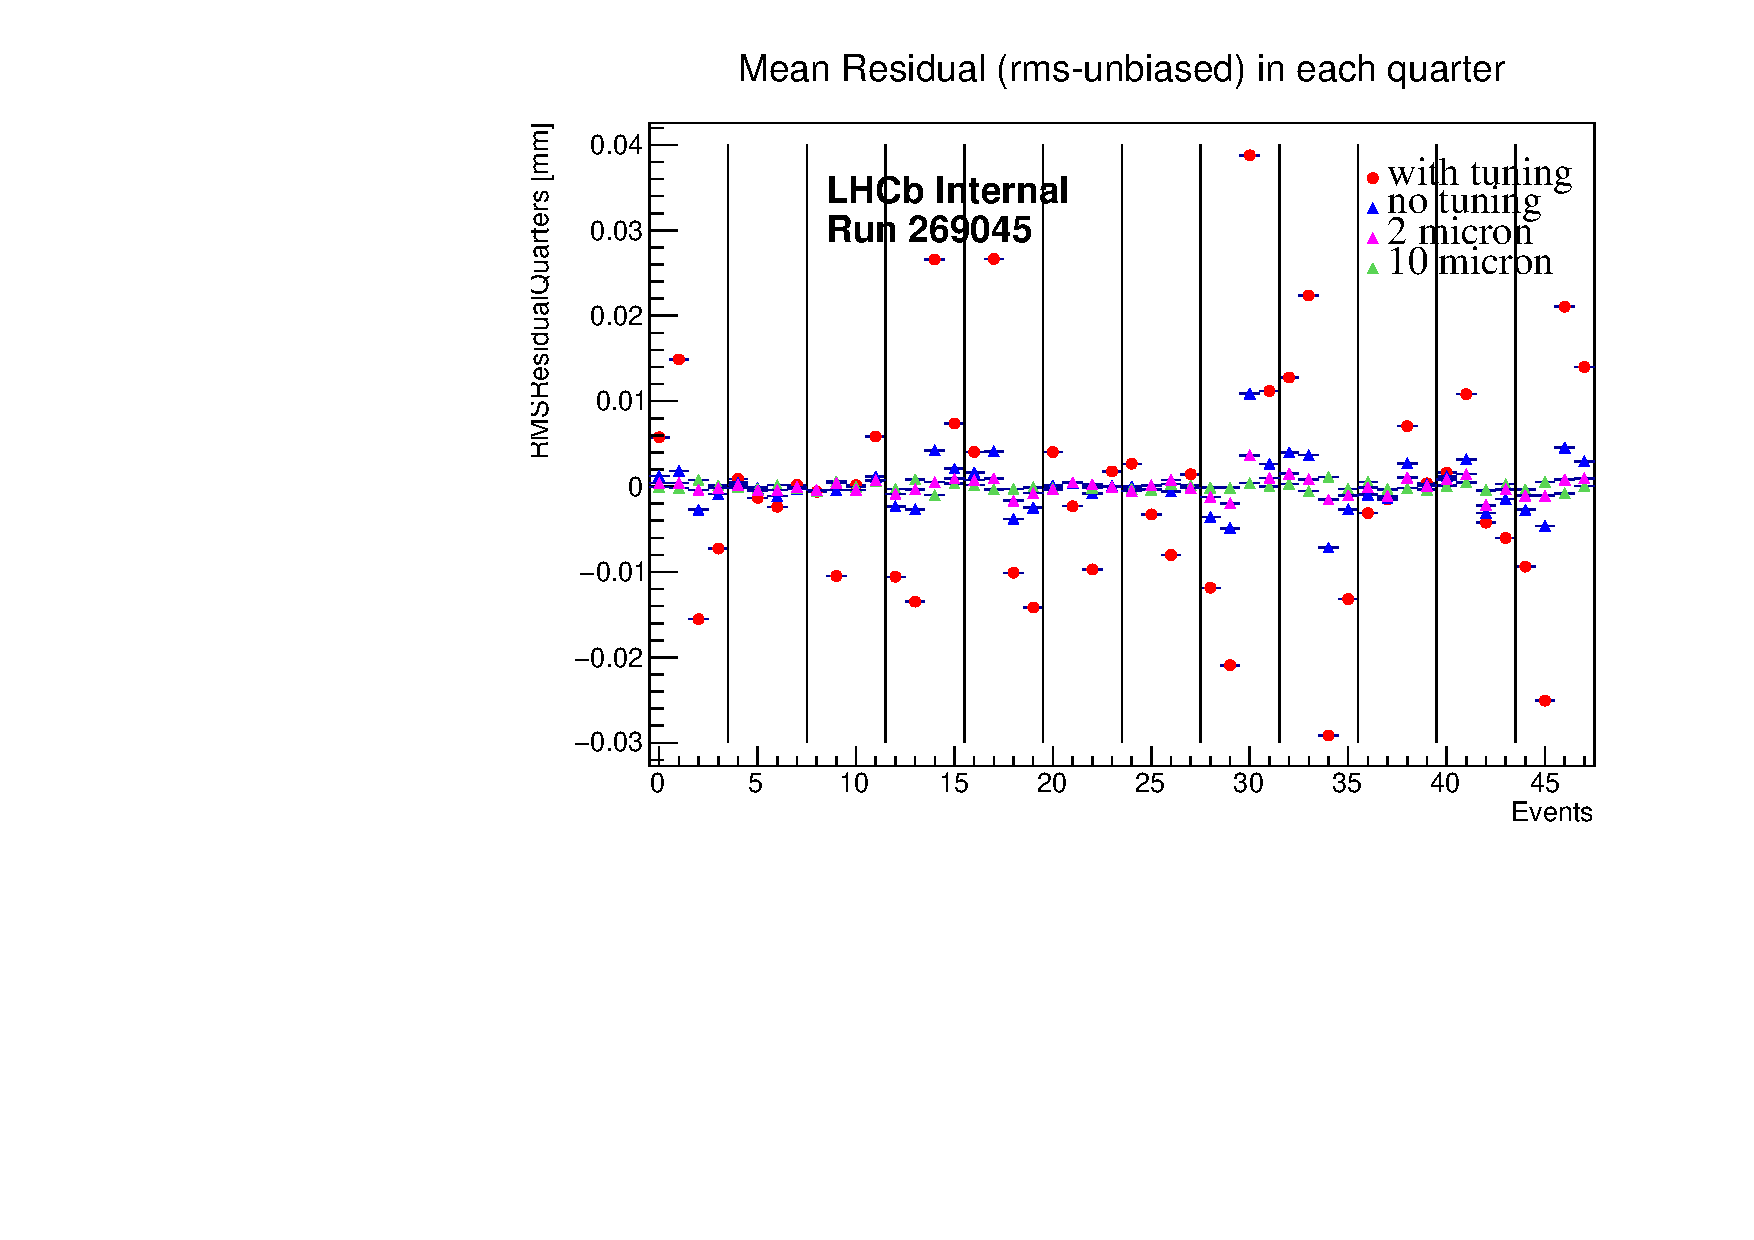
\includegraphics[width=\textwidth]{plots/compi/RMSResidualQuarterscomp_choice.pdf}
      \end{figure}
    \end{column}
    \begin{column}[c]{0.48\textwidth}
      \begin{figure}
        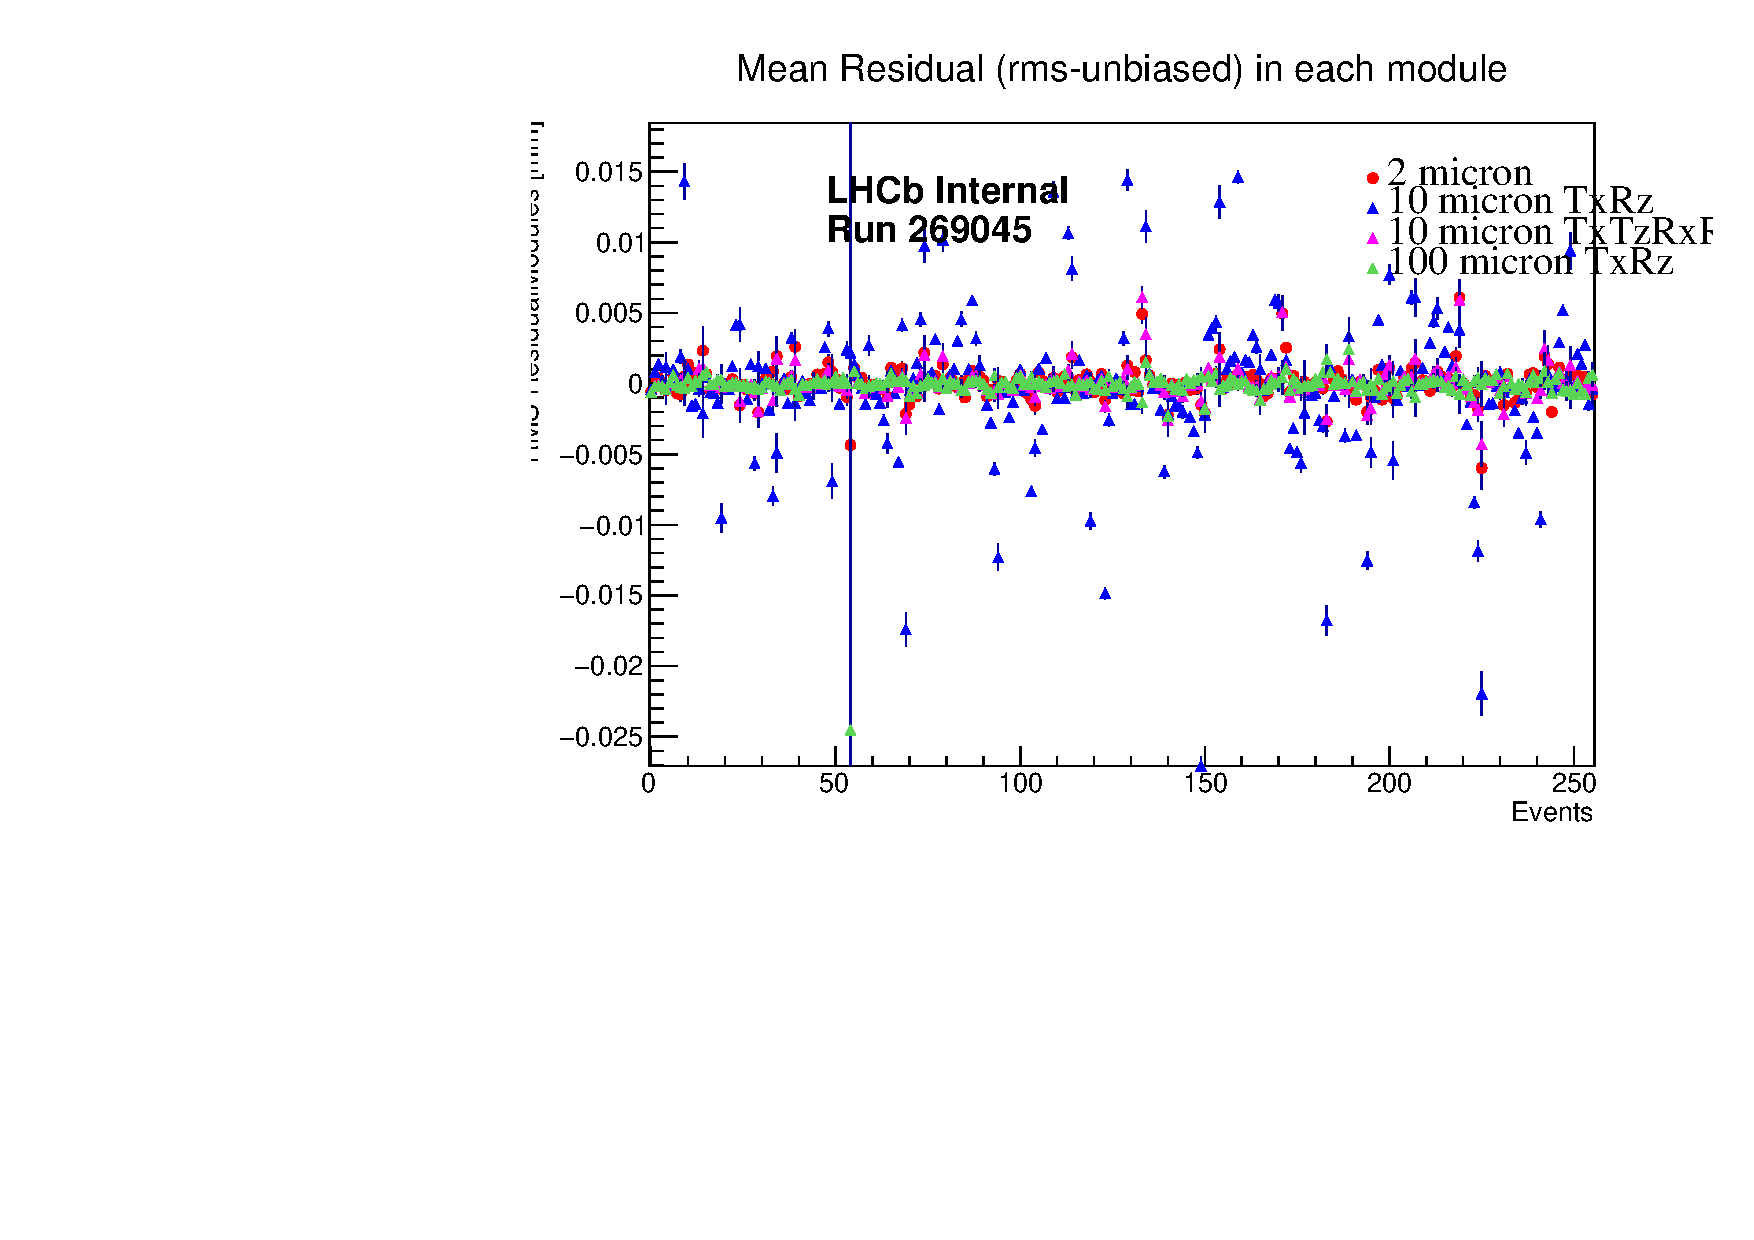
\includegraphics[width=\textwidth]{plots/compi/RMSResidualModulescomp_choice.pdf}
      \end{figure}
    \end{column}
  \end{columns}
\end{frame}

\begin{frame}\frametitle{T1 constants}
  \begin{columns}
    \begin{column}[c]{0.5\textwidth}
      \begin{figure}
        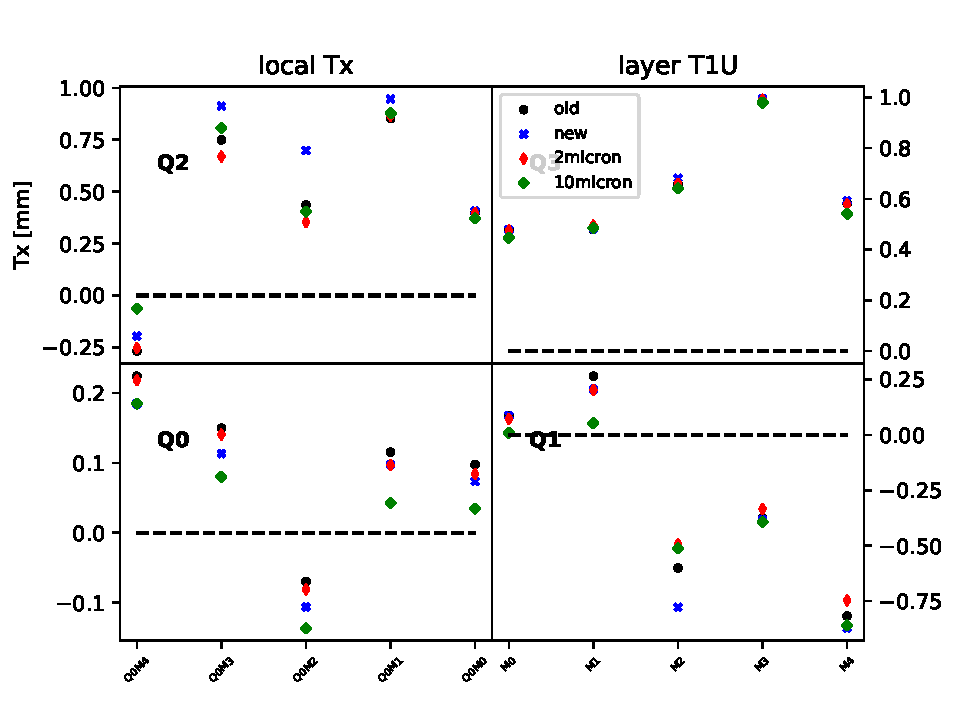
\includegraphics[width=0.6\textwidth]{plots/compi/Tx/blue_red_comp_T1U_Tx.pdf}
        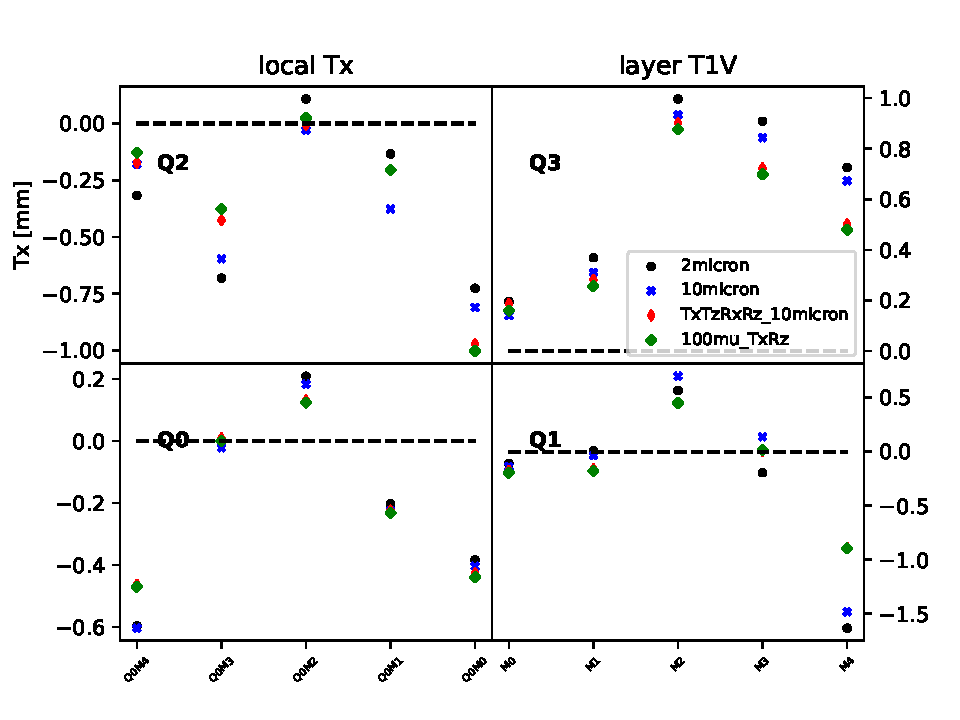
\includegraphics[width=0.6\textwidth]{plots/compi/Tx/blue_red_comp_T1V_Tx.pdf}
      \end{figure}
    \end{column}
    \begin{column}[c]{0.5\textwidth}
      \begin{figure}
        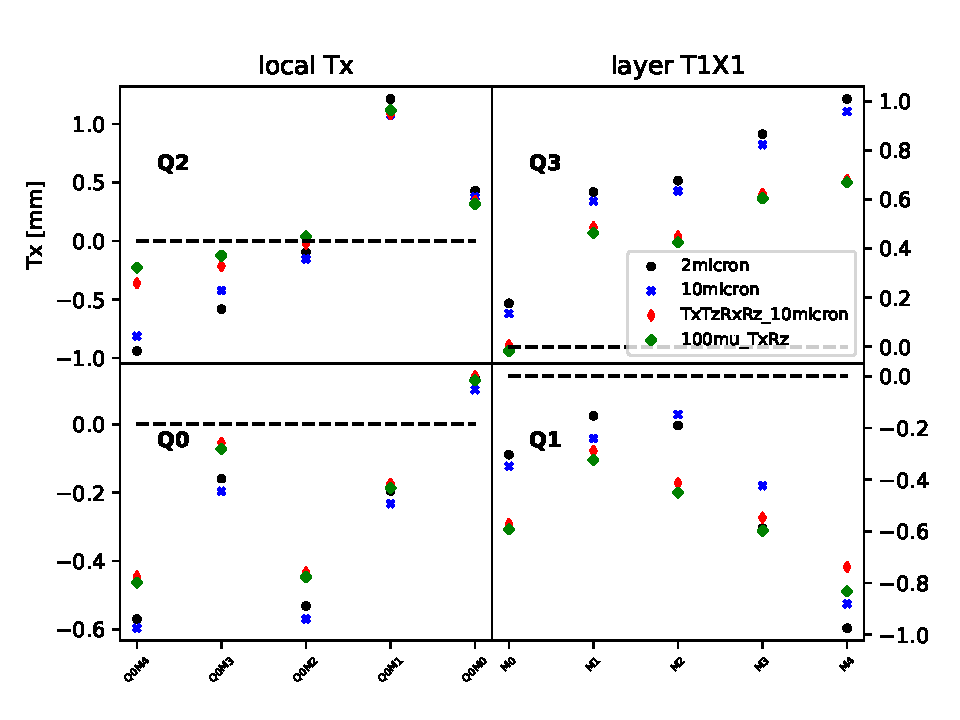
\includegraphics[width=0.6\textwidth]{plots/compi/Tx/blue_red_comp_T1X1_Tx.pdf}
        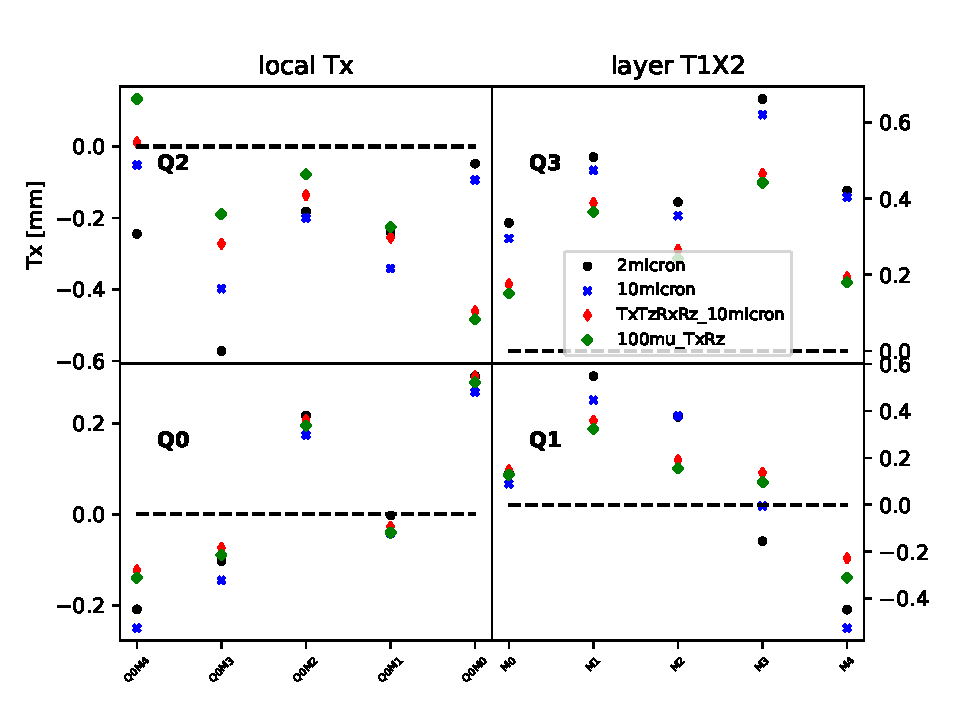
\includegraphics[width=0.6\textwidth]{plots/compi/Tx/blue_red_comp_T1X2_Tx.pdf}
      \end{figure}
    \end{column}
  \end{columns}
\end{frame}

\begin{frame}\frametitle{T2 constants}
  \begin{columns}
    \begin{column}[c]{0.5\textwidth}
      \begin{figure}
        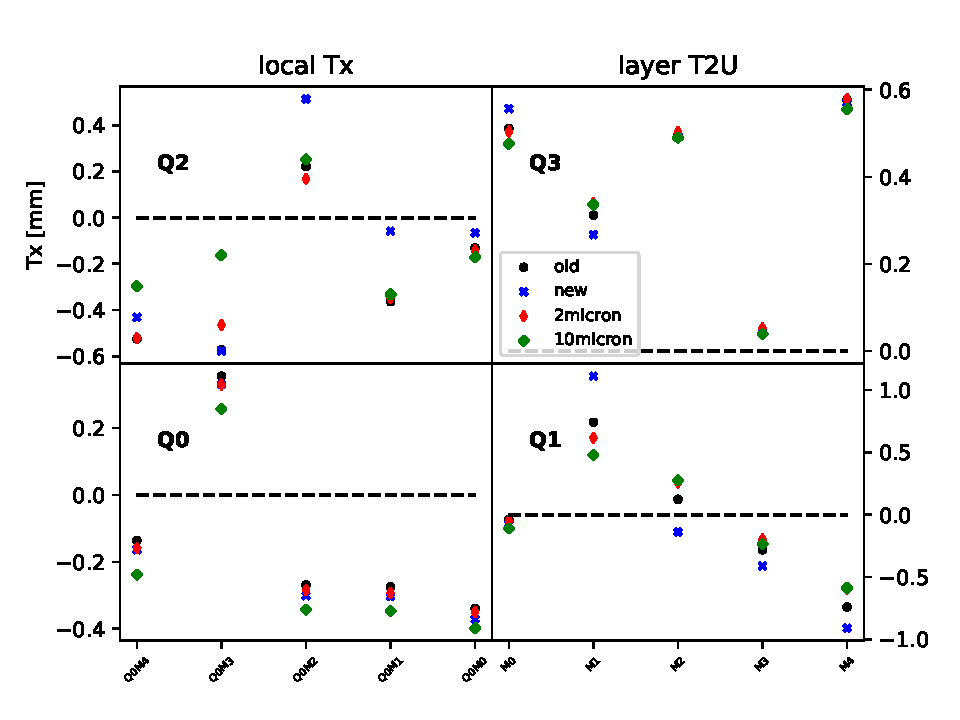
\includegraphics[width=0.6\textwidth]{plots/compi/Tx/blue_red_comp_T2U_Tx.pdf}
        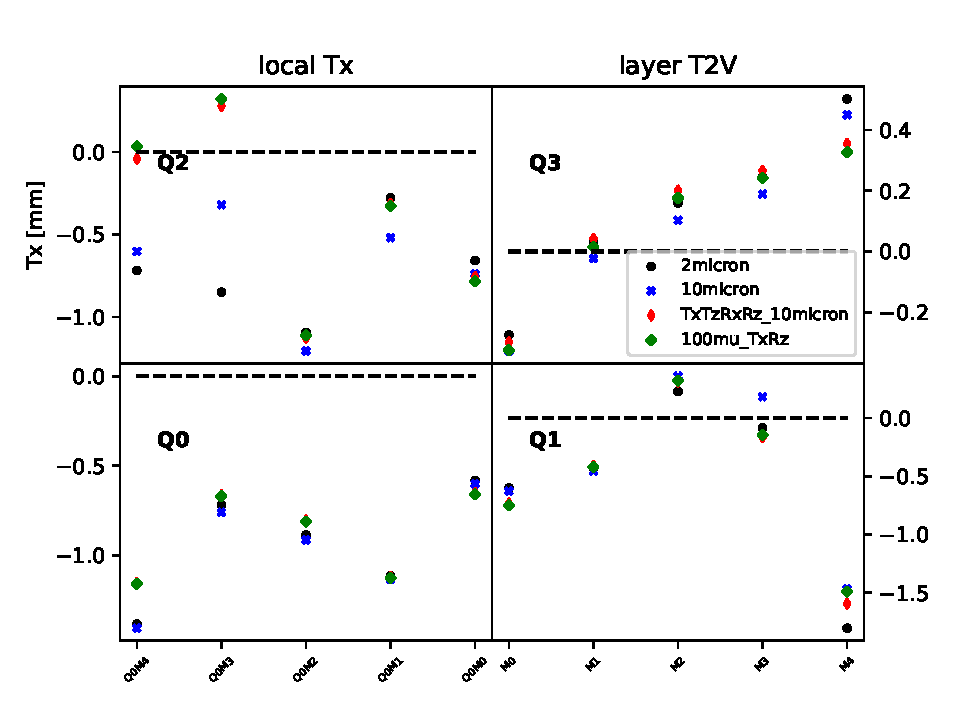
\includegraphics[width=0.6\textwidth]{plots/compi/Tx/blue_red_comp_T2V_Tx.pdf}
      \end{figure}
    \end{column}
    \begin{column}[c]{0.5\textwidth}
      \begin{figure}
        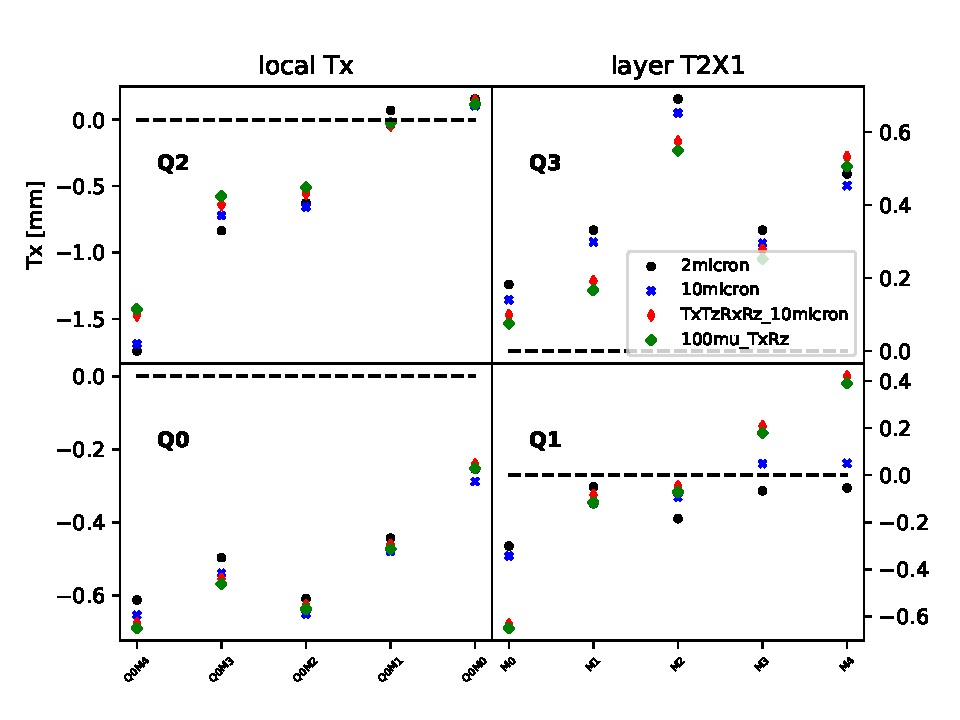
\includegraphics[width=0.6\textwidth]{plots/compi/Tx/blue_red_comp_T2X1_Tx.pdf}
        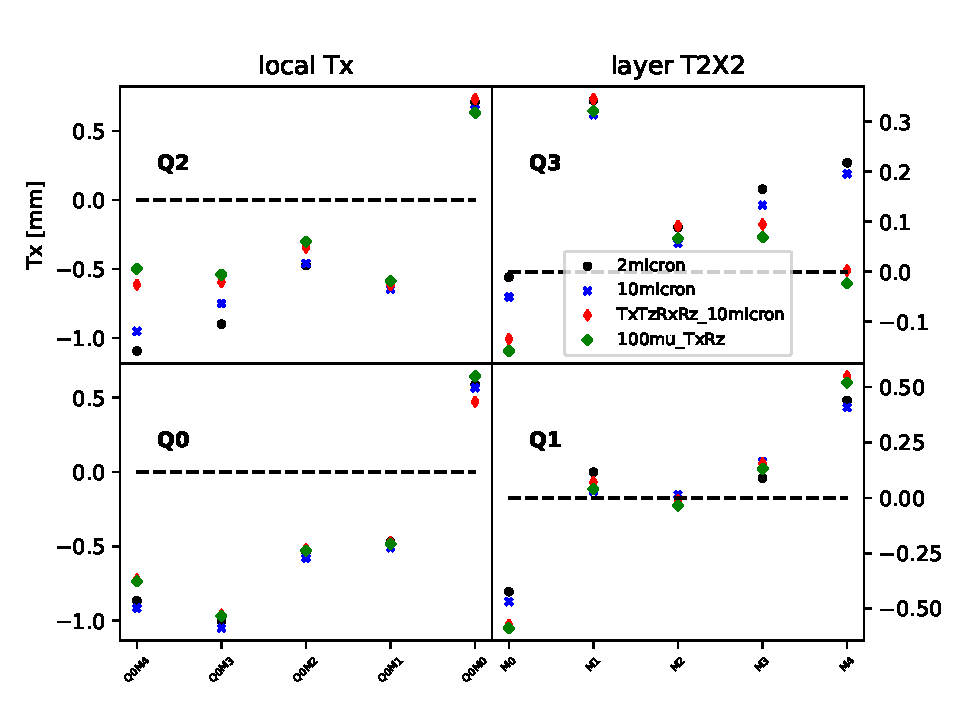
\includegraphics[width=0.6\textwidth]{plots/compi/Tx/blue_red_comp_T2X2_Tx.pdf}
      \end{figure}
    \end{column}
  \end{columns}
\end{frame}

\begin{frame}\frametitle{T3 constants}
  \begin{columns}
    \begin{column}[c]{0.5\textwidth}
      \begin{figure}
        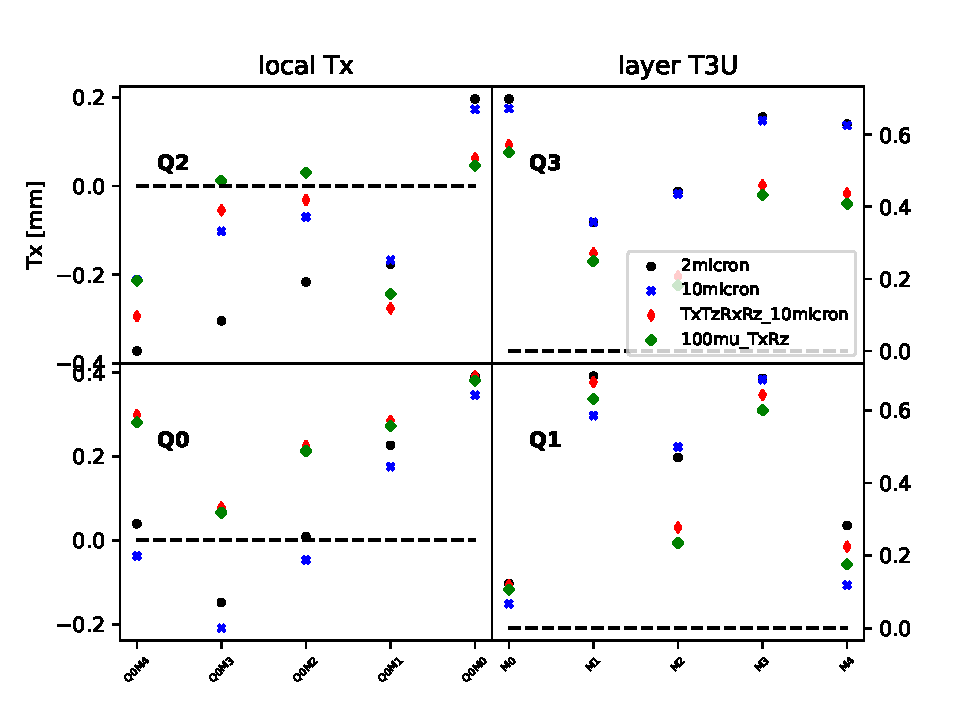
\includegraphics[width=0.6\textwidth]{plots/compi/Tx/blue_red_comp_T3U_Tx.pdf}
        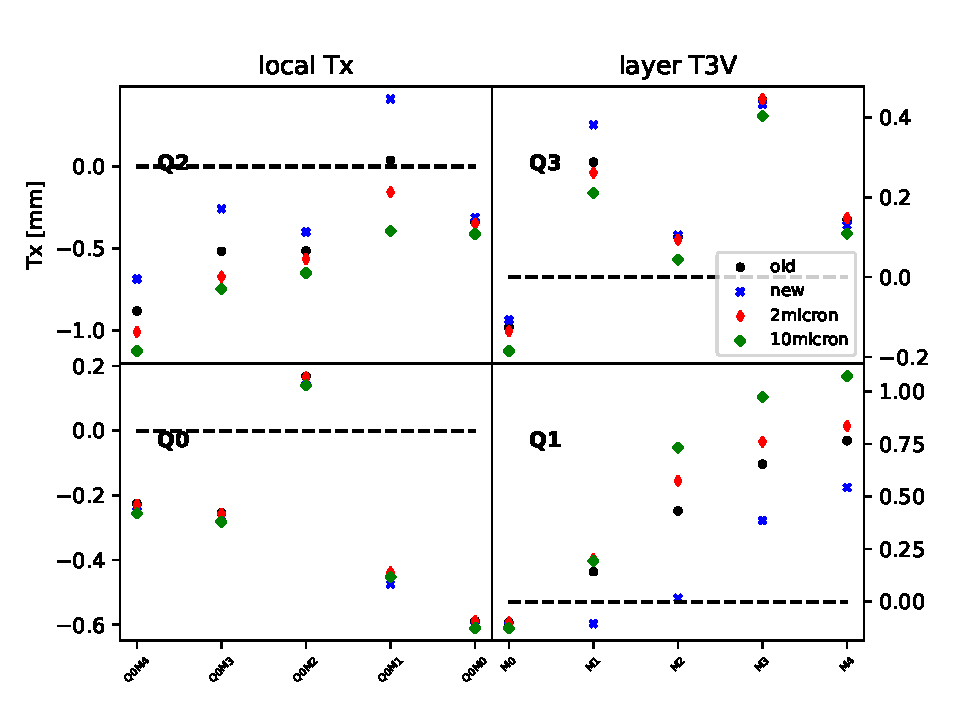
\includegraphics[width=0.6\textwidth]{plots/compi/Tx/blue_red_comp_T3V_Tx.pdf}
      \end{figure}
    \end{column}
    \begin{column}[c]{0.5\textwidth}
      \begin{figure}
        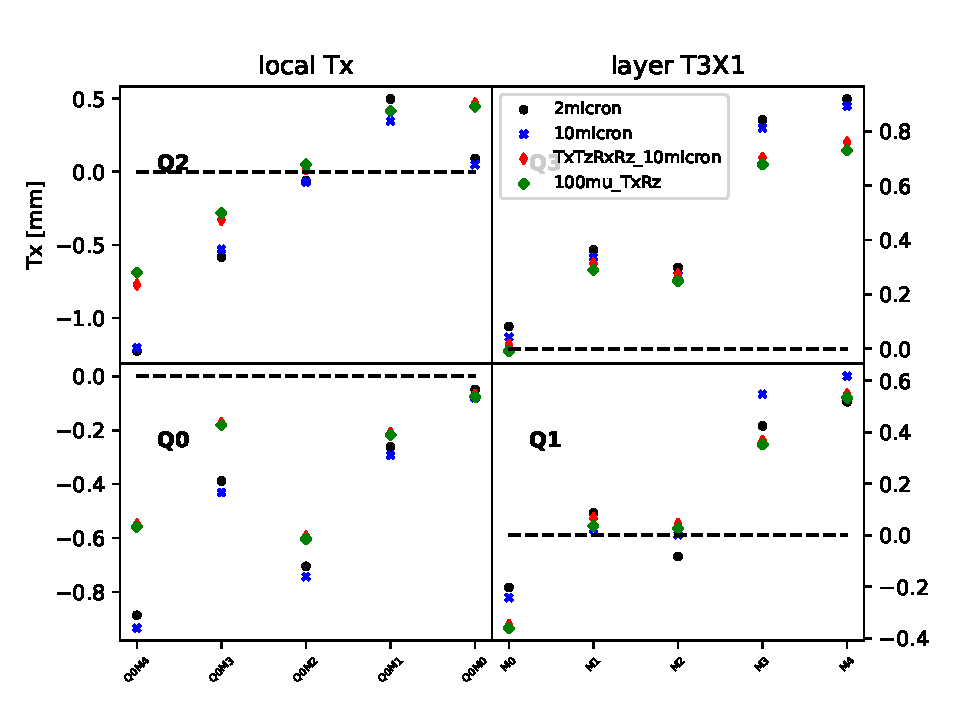
\includegraphics[width=0.6\textwidth]{plots/compi/Tx/blue_red_comp_T3X1_Tx.pdf}
        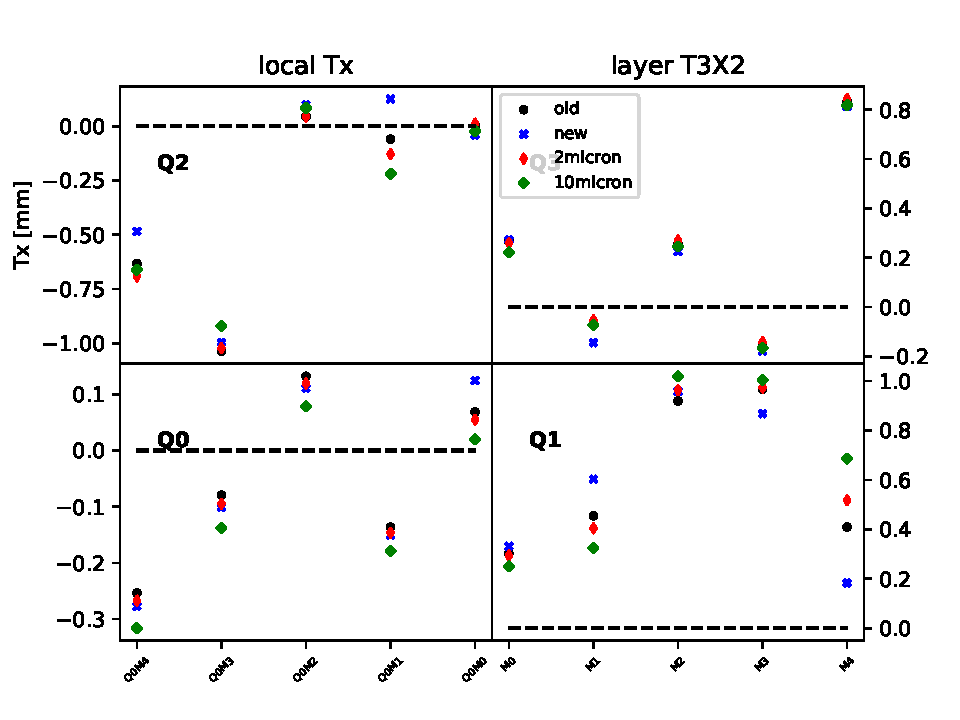
\includegraphics[width=0.6\textwidth]{plots/compi/Tx/blue_red_comp_T3X2_Tx.pdf}
      \end{figure}
    \end{column}
  \end{columns}
\end{frame}

\begin{frame}
  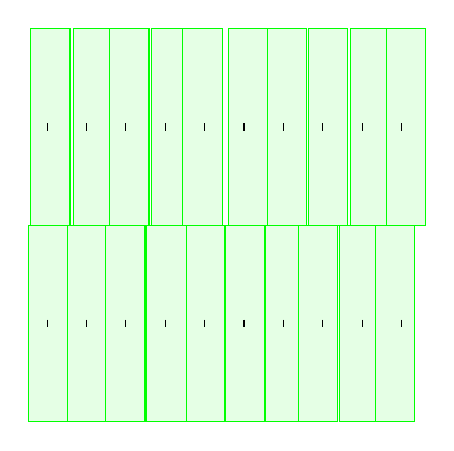
\begin{tikzpicture}
    % top modules
    % Q 2, 0.3982    0.8524    0.4359    0.7492   -0.2673
    \node[rectangle, 
    draw = green, 
    fill = green!10!white, 
    minimum width = 0.5cm, 
    minimum height = 2.5cm] (r) at (0 + 0.03982,1.25) {};
    \node[rectangle, 
    draw = green, 
    fill = green!10!white, 
    minimum width = 0.5cm, 
    minimum height = 2.5cm] (r) at (0.5 + 0.08524,1.25) {};
    \node[rectangle, 
    draw = green, 
    fill = green!10!white, 
    minimum width = 0.5cm, 
    minimum height = 2.5cm] (r) at (1 + 0.04359,1.25) {};
    \node[rectangle, 
    draw = green, 
    fill = green!10!white, 
    minimum width = 0.5cm, 
    minimum height = 2.5cm] (r) at (1.5 + 0.07492,1.25) {};
    \node[rectangle, 
    draw = green, 
    fill = green!10!white, 
    minimum width = 0.5cm, 
    minimum height = 2.5cm] (r) at (2 - 0.02673,1.25) {};

    % Q 3, 0.4769    0.4792    0.6595    0.9835    0.5815
    \node[rectangle, 
    draw = green, 
    fill = green!10!white, 
    minimum width = 0.5cm, 
    minimum height = 2.5cm] (r) at (2.5 + 0.04769,1.25) {};
    \node[rectangle, 
    draw = green, 
    fill = green!10!white, 
    minimum width = 0.5cm, 
    minimum height = 2.5cm] (r) at (3 + 0.04792,1.25) {};
    \node[rectangle, 
    draw = green, 
    fill = green!10!white, 
    minimum width = 0.5cm, 
    minimum height = 2.5cm] (r) at (3.5 + 0.06595,1.25) {};
    \node[rectangle, 
    draw = green, 
    fill = green!10!white, 
    minimum width = 0.5cm, 
    minimum height = 2.5cm] (r) at (4 + 0.09835,1.25) {};
    \node[rectangle, 
    draw = green, 
    fill = green!10!white, 
    minimum width = 0.5cm, 
    minimum height = 2.5cm] (r) at (4.5 + 0.05815,1.25) {};

    % bottom modules
    % Q 0, 0.09739   0.1152   -0.06989   0.1495    0.224
    \node[rectangle, 
    draw = green, 
    fill = green!10!white, 
    minimum width = 0.5cm, 
    minimum height = 2.5cm] (r) at (0 + 0.009739,-1.25) {};
    \node[rectangle, 
    draw = green, 
    fill = green!10!white, 
    minimum width = 0.5cm, 
    minimum height = 2.5cm] (r) at (0.5 + 0.01152,-1.25) {};
    \node[rectangle, 
    draw = green, 
    fill = green!10!white, 
    minimum width = 0.5cm, 
    minimum height = 2.5cm] (r) at (1 - 0.006989,-1.25) {};
    \node[rectangle, 
    draw = green, 
    fill = green!10!white, 
    minimum width = 0.5cm, 
    minimum height = 2.5cm] (r) at (1.5 + 0.01495,-1.25) {};
    \node[rectangle, 
    draw = green, 
    fill = green!10!white, 
    minimum width = 0.5cm, 
    minimum height = 2.5cm] (r) at (2 + 0.0224,-1.25) {};

    % Q 1, 0.08787   0.2648   -0.6002   -0.3735   -0.8177
    \node[rectangle, 
    draw = green, 
    fill = green!10!white, 
    minimum width = 0.5cm, 
    minimum height = 2.5cm] (r) at (2.5 + 0.008787,-1.25) {};
    \node[rectangle, 
    draw = green, 
    fill = green!10!white, 
    minimum width = 0.5cm, 
    minimum height = 2.5cm] (r) at (3 + 0.02648,-1.25) {};
    \node[rectangle, 
    draw = green, 
    fill = green!10!white, 
    minimum width = 0.5cm, 
    minimum height = 2.5cm] (r) at (3.5 - 0.06002,-1.25) {};
    \node[rectangle, 
    draw = green, 
    fill = green!10!white, 
    minimum width = 0.5cm, 
    minimum height = 2.5cm] (r) at (4 - 0.03735,-1.25) {};
    \node[rectangle, 
    draw = green, 
    fill = green!10!white, 
    minimum width = 0.5cm, 
    minimum height = 2.5cm] (r) at (4.5 - 0.08177,-1.25) {};

    \draw (0, 1.2)   -- (0, 1.3);
    \draw (0.5, 1.2) -- (0.5, 1.3);
    \draw (1, 1.2)   -- (1, 1.3);
    \draw (1.5, 1.2) -- (1.5, 1.3);
    \draw (2, 1.2)   -- (2, 1.3);
    \draw (2.5, 1.2) -- (2.5, 1.3);
    \draw (3, 1.2)   -- (3, 1.3);
    \draw (3.5, 1.2) -- (3.5, 1.3);
    \draw (4, 1.2)   -- (4, 1.3);
    \draw (4.5, 1.2) -- (4.5, 1.3);

    \draw (0, -1.2)   -- (0, -1.3);
    \draw (0.5, -1.2) -- (0.5, -1.3);
    \draw (1, -1.2)   -- (1, -1.3);
    \draw (1.5, -1.2) -- (1.5, -1.3);
    \draw (2, -1.2)   -- (2, -1.3);
    \draw (2.5, -1.2) -- (2.5, -1.3);
    \draw (3, -1.2)   -- (3, -1.3);
    \draw (3.5, -1.2) -- (3.5, -1.3);
    \draw (4, -1.2)   -- (4, -1.3);
    \draw (4.5, -1.2) -- (4.5, -1.3);

    % 10 micron
    % top modules
    % Q 2, 0.3721    0.8772   0.4041    0.8068   -0.06332 
    % \node[rectangle, 
    % draw = red, 
    % fill = red!10!white, 
    % minimum width = 0.5cm, 
    % minimum height = 2.5cm] (r) at (5 + 0.03721,1.25) {};
    % \node[rectangle, 
    % draw = red, 
    % fill = red!10!white, 
    % minimum width = 0.5cm, 
    % minimum height = 2.5cm] (r) at (5.5 + 0.08772,1.25) {};
    % \node[rectangle, 
    % draw = red, 
    % fill = red!10!white, 
    % minimum width = 0.5cm, 
    % minimum height = 2.5cm] (r) at (6 + 0.04041,1.25) {};
    % \node[rectangle, 
    % draw = red, 
    % fill = red!10!white, 
    % minimum width = 0.5cm, 
    % minimum height = 2.5cm] (r) at (6.5 + 0.08068,1.25) {};
    % \node[rectangle, 
    % draw = red, 
    % fill = red!10!white, 
    % minimum width = 0.5cm, 
    % minimum height = 2.5cm] (r) at (7 - 0.006332,1.25) {};

    % % Q 3, 0.4462    0.485     0.6413    0.9798    0.5411 
    % \node[rectangle, 
    % draw = red, 
    % fill = red!10!white, 
    % minimum width = 0.5cm, 
    % minimum height = 2.5cm] (r) at (7.5 + 0.04462,1.25) {};
    % \node[rectangle, 
    % draw = red, 
    % fill = red!10!white, 
    % minimum width = 0.5cm, 
    % minimum height = 2.5cm] (r) at (8 + 0.0485,1.25) {};
    % \node[rectangle, 
    % draw = red, 
    % fill = red!10!white, 
    % minimum width = 0.5cm, 
    % minimum height = 2.5cm] (r) at (8.5 + 0.06413,1.25) {};
    % \node[rectangle, 
    % draw = red, 
    % fill = red!10!white, 
    % minimum width = 0.5cm, 
    % minimum height = 2.5cm] (r) at (9 + 0.09798,1.25) {};
    % \node[rectangle, 
    % draw = red, 
    % fill = red!10!white, 
    % minimum width = 0.5cm, 
    % minimum height = 2.5cm] (r) at (9.5 + 0.05411,1.25) {};

    % % bottom modules
    % % Q 0, 0.03441   0.0422   -0.1366    0.08028   0.1846 
    % \node[rectangle, 
    % draw = red, 
    % fill = red!10!white, 
    % minimum width = 0.5cm, 
    % minimum height = 2.5cm] (r) at (5 + 0.003441,-1.25) {};
    % \node[rectangle, 
    % draw = red, 
    % fill = red!10!white, 
    % minimum width = 0.5cm, 
    % minimum height = 2.5cm] (r) at (5.5 + 0.00422,-1.25) {};
    % \node[rectangle, 
    % draw = red, 
    % fill = red!10!white, 
    % minimum width = 0.5cm, 
    % minimum height = 2.5cm] (r) at (6 - 0.01366,-1.25) {};
    % \node[rectangle, 
    % draw = red, 
    % fill = red!10!white, 
    % minimum width = 0.5cm, 
    % minimum height = 2.5cm] (r) at (6.5 + 0.008028,-1.25) {};
    % \node[rectangle, 
    % draw = red, 
    % fill = red!10!white, 
    % minimum width = 0.5cm, 
    % minimum height = 2.5cm] (r) at (7 + 0.01846,-1.25) {};

    % % Q 1, 0.008918  0.05205  -0.5124   -0.3931   -0.8599
    % \node[rectangle, 
    % draw = red, 
    % fill = red!10!white, 
    % minimum width = 0.5cm, 
    % minimum height = 2.5cm] (r) at (7.5 + 0.0008918,-1.25) {};
    % \node[rectangle, 
    % draw = red, 
    % fill = red!10!white, 
    % minimum width = 0.5cm, 
    % minimum height = 2.5cm] (r) at (8 + 0.005205,-1.25) {};
    % \node[rectangle, 
    % draw = red, 
    % fill = red!10!white, 
    % minimum width = 0.5cm, 
    % minimum height = 2.5cm] (r) at (8.5 - 0.05124,-1.25) {};
    % \node[rectangle, 
    % draw = red, 
    % fill = red!10!white, 
    % minimum width = 0.5cm, 
    % minimum height = 2.5cm] (r) at (9 - 0.03931,-1.25) {};
    % \node[rectangle, 
    % draw = red, 
    % fill = red!10!white, 
    % minimum width = 0.5cm, 
    % minimum height = 2.5cm] (r) at (9.5 - 0.08599,-1.25) {};

    % \node[draw, align=left] at (0.5, 4.1) {top half module};
    % \node[draw, align=left] at (1, 1.25) {joint};
    % \node[draw, align=left] at (0.5, -1.55) {bottom half module};
\end{tikzpicture}

% old
% [ 0.09739   0.1152   -0.06989   0.1495    0.224
    % 0.3982    0.8524    0.4359    0.7492   -0.2673
    % 0.08787   0.2648   -0.6002   -0.3735   -0.8177
    % 0.4769    0.4792    0.6595    0.9835    0.5815  ]

% tuned
% [ 0.07349   0.09724  -0.106     0.1132    0.1847    0.4075    0.9464
%    0.6986    0.9121   -0.1961    0.08715   0.2053   -0.7778   -0.3823
%   -0.8722    0.4787    0.4822    0.6807    0.9938    0.5928  ]

% 2 micron
% [ 0.08396   0.09674  -0.0814    0.1405    0.2181    0.3974    0.8662
%    0.353     0.6693   -0.2526    0.07106   0.2024   -0.4929   -0.334
%   -0.7467    0.4746    0.4947    0.6599    0.9914    0.5784  ]

% 10 micron
% [ 0.03441   0.0422   -0.1366    0.08028   0.1846    
%   0.3721    0.8772   0.4041    0.8068   -0.06332 
%   0.008918  0.05205  -0.5124   -0.3931   -0.8599  
%   0.4462    0.485     0.6413    0.9798    0.5411  ]
\end{frame}

\end{document}
